\documentclass[aspectratio=169,11pt]{beamer}

% ============================================================
% PACKAGES
% ============================================================
\usepackage{graphicx}
\usepackage{tikz}
\usetikzlibrary{positioning,arrows.meta}
\usepackage{xcolor}
\usepackage{booktabs}
\usepackage{tabularx}
\usepackage{array}
\usepackage{ragged2e}
\usepackage{hyperref}

% ============================================================
% COLORS - SAME AS PHASE-I
% ============================================================
\definecolor{GEUBlue}{RGB}{20,55,105}
\definecolor{GEULightBlue}{RGB}{238,244,251}
\definecolor{GEUGrey}{RGB}{90,90,90}
\definecolor{GEULightGrey}{RGB}{245,246,248}

% ============================================================
% BEAMER SETTINGS
% ============================================================
\usetheme{default}
\setbeamertemplate{navigation symbols}{}
\setbeamertemplate{blocks}[rounded][shadow=false]

\setbeamercolor{normal text}{fg=black,bg=white}
\setbeamercolor{frametitle}{fg=GEUBlue}
\setbeamercolor{structure}{fg=GEUBlue}
\setbeamercolor{block title}{fg=GEUBlue,bg=GEULightBlue}
\setbeamercolor{block body}{fg=black,bg=GEULightBlue}

\setbeamerfont{frametitle}{size=\Large,series=\bfseries}

% ============================================================
% LOGO
% ============================================================
% Upload the Graphic Era logo with this filename to Overleaf.
\newcommand{\GEULogo}{graphicera_logo.png}

% ============================================================
% HEADER
% ============================================================
\setbeamertemplate{headline}{%
  \begin{tikzpicture}[remember picture,overlay]
    \node[
        anchor=north east,
        xshift=-0.30cm,
        yshift=-0.12cm
    ] at (current page.north east)
    {\IfFileExists{\GEULogo}{\includegraphics[height=0.62cm]{\GEULogo}}{}};
  \end{tikzpicture}
  \vspace{0.72cm}
}

% ============================================================
% FRAME TITLE
% ============================================================
\setbeamertemplate{frametitle}{%
  \vspace{0.03cm}
  \insertframetitle\par
  \vspace{0.04cm}
  \textcolor{GEUBlue}{\rule{\textwidth}{0.9pt}}
  \vspace{0.03cm}
}

% ============================================================
% FOOTER
% ============================================================
\setbeamertemplate{footline}{%
  \leavevmode
  \hbox{%
  \begin{beamercolorbox}[
      wd=.82\paperwidth,
      ht=0.32cm,
      dp=0.10cm,
      leftskip=.3cm
  ]{author in head/foot}
    \tiny Department of Computer Science \& Engineering |
    Graphic Era (Deemed to be University)
  \end{beamercolorbox}%
  \begin{beamercolorbox}[
      wd=.18\paperwidth,
      ht=0.32cm,
      dp=0.10cm,
      rightskip=.3cm
  ]{date in head/foot}
    \hfill\tiny\insertframenumber/\inserttotalframenumber
  \end{beamercolorbox}}
}

% ============================================================
% CUSTOM COMMANDS
% ============================================================
\newcommand{\smallnote}[1]{%
\vspace{0.08cm}
{\scriptsize\color{GEUGrey}#1}
}

\newcommand{\placeholder}[1]{%
\textit{\color{GEUGrey}#1}
}

% ============================================================
% DOCUMENT INFORMATION
% ============================================================
\title{\textbf{Project-Based Learning}\\[2mm]\large Phase-II Evaluation}
\author{\textbf{Smart Driver Drowsiness \& Safety System}\\Team ID: DSCPP-III-2026-T234}

\institute{
Department of Computer Science \& Engineering\\
Graphic Era (Deemed to be University), Dehradun
}

\date{Academic Session 2026--27}

% ============================================================
% DOCUMENT
% ============================================================
\begin{document}

% ============================================================
% SLIDE 1
% ============================================================
\begin{frame}[plain]

\begin{tikzpicture}[remember picture,overlay]

\draw[GEUBlue,line width=3pt]
(current page.north west) -- (current page.north east);

\node[
    anchor=north east,
    xshift=-0.45cm,
    yshift=-0.35cm
] at (current page.north east)
{\IfFileExists{\GEULogo}{\includegraphics[height=1.0cm]{\GEULogo}}{}};

\node[
    align=center,
    text width=.84\paperwidth
] at ([yshift=.25cm]current page.center)
{
{\color{GEUBlue}
\fontsize{26}{30}\selectfont
\bfseries PROJECT-BASED LEARNING}
\\[3mm]

{\fontsize{18}{22}\selectfont
PHASE-II EVALUATION}
\\[7mm]

{\color{GEUGrey}
\Large\bfseries
\placeholder{Smart Driver Drowsiness \& Safety System}}
\\[3mm]

{\color{GEUBlue}
\normalsize Team ID: DSCPP-III-2026-T234}
};

\node[
    align=center,
    anchor=south,
    yshift=.42cm
] at (current page.south)
{
\bfseries
Department of Computer Science \& Engineering\\
Graphic Era (Deemed to be University), Dehradun\\[-1mm]
\scriptsize Academic Session 2026--27
};

\end{tikzpicture}

\end{frame}

% ============================================================
% SLIDE 2
% ============================================================
\begin{frame}{Team \& Mentor Details}

\begin{columns}[T,totalwidth=\textwidth]

\column{.48\textwidth}

\begin{block}{Team Information}
\begin{tabular}{@{}ll@{}}
\textbf{Team ID:} & DSCPP-III-2026-T234\\
\textbf{Semester:} & 3rd\\
\textbf{Section:} & H, E, ML4, ML3\\
\textbf{Domain:} & \placeholder{Computer Vision \& Safety}
\end{tabular}
\end{block}

\column{.48\textwidth}

\begin{block}{Team Members}
1.\quad \placeholder{Ridvik Garg -- 2028039}\\
2.\quad \placeholder{Prabhav Gulyani -- 2027975}\\
3.\quad \placeholder{Nandini Gupta -- 2028777}\\
4.\quad \placeholder{Antriksh Gehlot -- 2028648}
\end{block}

\end{columns}

\vspace{2mm}

\begin{block}{Mentor}
\placeholder{Mr. Kamal Kumar Gola}
\hfill
\textbf{Interactions completed:}
\underline{\hspace{4mm}04\hspace{4mm}}
\end{block}

\vfill

\smallnote{
Brief Discussion: Introduce the team, project domain, mentor,
and responsibilities of the team members.
}

\end{frame}

% ============================================================
% SLIDE 3
% ============================================================
\begin{frame}{Phase-I Recap \& Feedback Incorporated}

\begin{block}{Phase-I Status}
\placeholder{
Proposed a webcam system to track driver eyes and head position to prevent accidents from sleepy drivers.
}
\end{block}

\vspace{2mm}

\begin{columns}[T,totalwidth=\textwidth]

\column{.48\textwidth}

\textbf{\color{GEUBlue}Feedback Received}

\begin{itemize}\itemsep2pt
\item \placeholder{Use proper DSA instead of standard vectors}
\item \placeholder{Split project into smaller testable modules}
\item \placeholder{Avoid false beeps on normal eye blinks}
\end{itemize}

\column{.48\textwidth}

\textbf{\color{GEUBlue}Changes Incorporated}

\begin{itemize}\itemsep2pt
\item \placeholder{Added Queue, Stack, and Linked List classes}
\item \placeholder{Divided code into Vision, DSA, and DB modules}
\item \placeholder{Checked longer eye closure before alerting}
\end{itemize}

\end{columns}

\vfill

\smallnote{
Brief Discussion: Explain the major feedback received during Phase-I
and clearly demonstrate how it has been incorporated.
}

\end{frame}

% ============================================================
% SLIDE 4
% ============================================================
\begin{frame}{Problem Statement \& Finalized Objectives}

\begin{block}{Problem Statement}
\placeholder{
Prevent accidents caused by sleepy drivers by tracking prolonged eye closure via webcam and giving step-by-step alerts.
}
\end{block}

\vspace{2mm}

\textbf{\color{GEUBlue}Finalized Objectives}

\begin{enumerate}\itemsep3pt
\item \placeholder{Capture live webcam video with OpenCV to check eye closure and head position.}
\item \placeholder{Use a Queue for incoming events, a Stack for recent alerts, and a Linked List for history.}
\item \placeholder{Play step-by-step sound alerts, lower car music volume, and send emergency SMS.}
\item \placeholder{Save all past safety events and logs inside a local SQLite database.}
\end{enumerate}

\vfill
\vspace{-2mm} % Pulls the note up slightly if needed
\smallnote{Brief Discussion: Avoid repeating the complete Phase-I presentation. Focus on the finalized problem, scope and measurable objectives.}
\end{frame}
\end{frame}

% ============================================================
% SLIDE 5
% ============================================================
\begin{frame}{Updated System Architecture / Workflow}

\begin{center}

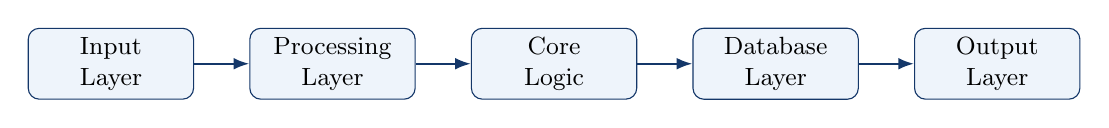
\begin{tikzpicture}[
node distance=7mm,
box/.style={
rectangle,
rounded corners,
draw=GEUBlue,
fill=GEULightBlue,
minimum width=2.10cm,
minimum height=9mm,
align=center,
font=\small
},
arrow/.style={
-{Latex[length=2mm]},
thick,
draw=GEUBlue
}
]

\node[box] (a) {Input\\Layer};
\node[box,right=of a] (b) {Processing\\Layer};
\node[box,right=of b] (c) {Core\\Logic};
\node[box,right=of c] (d) {Database\\Layer};
\node[box,right=of d] (e) {Output\\Layer};

\draw[arrow] (a)--(b);
\draw[arrow] (b)--(c);
\draw[arrow] (c)--(d);
\draw[arrow] (d)--(e);

\end{tikzpicture}

\end{center}

\vspace{4mm}

\begin{columns}[T,totalwidth=\textwidth]

\column{.48\textwidth}

\textbf{\color{GEUBlue}Major Components}

\begin{itemize}\itemsep2pt
\item \placeholder{OpenCV Camera \& Face Tracking}
\item \placeholder{C++ Queue, Stack \& Linked List Logic}
\item \placeholder{SQLite Database \& Alert Triggers}
\end{itemize}

\column{.48\textwidth}

\textbf{\color{GEUBlue}Changes Since Phase-I}

\begin{itemize}\itemsep2pt
\item \placeholder{Added custom DSA classes for events}
\item \placeholder{Added music mute and SMS features}
\item \placeholder{Split into separate testable modules}
\end{itemize}

\end{columns}

\vfill

\smallnote{
Brief Discussion: Present the updated architecture and explain
how individual modules communicate with each other.
}

\end{frame}

% ============================================================
% SLIDE 6 
% ============================================================
\begin{frame}{Module Design \& Functional Requirements}
\vspace{-2mm}
\begin{columns}[T, totalwidth=\textwidth]
\column{.48\textwidth}
\textbf{\color{GEUBlue}{Major Modules}}
\begin{enumerate}
\itemsep 0pt
\item \placeholder{Webcam \& OpenCV Vision Module}
\item \placeholder{C++ DSA Event Handler Module}
\item \placeholder{SQLite Database Storage Module}
\item \placeholder{Sound, Music Mute \& SMS Module}
\end{enumerate}

\column{.48\textwidth}
\textbf{\color{GEUBlue}{Functional Requirements}}
\begin{itemize}
\itemsep 0pt
\item \placeholder{Track eyes and verify prolonged closure}
\item \placeholder{Push events to Queue and alerts to Stack}
\item \placeholder{Save event history in Linked List \& DB}
\item \placeholder{Trigger beep, loud alarm, mute, and SMS}
\end{itemize}
\end{columns}

\vspace{1mm}
\begin{block}{Module Dependency}
\placeholder{OpenCV spots eye closure and sends events to the C++ Queue, which updates the Stack, triggers alerts, and saves logs to SQLite.}
\end{block}

\vspace{-1mm}
\smallnote{Brief Discussion: Explain what each module does and how it contributes to the complete system.}
\end{frame}

% ============================================================
% SLIDE 7
% ============================================================
\begin{frame}{Technology Stack \& Development Methodology}

\begin{columns}[T,totalwidth=\textwidth]

\column{.48\textwidth}

\begin{block}{Technology Stack}

\begin{itemize}\itemsep2pt
\item Programming: \placeholder{C++}
\item Database: \placeholder{SQLite}
\item Framework: \placeholder{OpenCV}
\item Development Tool: \placeholder{VS Code \& GCC}
\item Version Control: \placeholder{Git / GitHub}
\end{itemize}

\end{block}

\column{.48\textwidth}

\begin{block}{Development Methodology}

\begin{enumerate}\itemsep2pt
\item Requirement Analysis
\item System Design
\item Module Development
\item Integration
\item Testing \& Validation
\end{enumerate}

\end{block}

\end{columns}

\vfill

\smallnote{
Brief Discussion: Explain why the selected technologies are appropriate
and how the team is following the development methodology.
}

\end{frame}

% ============================================================
% ============================================================
% SLIDE 8 
% ============================================================
\begin{frame}{Implementation of PBL Course Concepts}
\scriptsize
\begin{center}
\renewcommand{\arraystretch}{1.25}
\begin{tabularx}{.96\textwidth}{@{} >{\bfseries} p{3.0cm} X p{2.5cm} @{}}
\toprule
Course & Concepts Actually Implemented & Project Module \\ 
\midrule
Data Structures in C & \placeholder{Queue (event order), Stack (recent alerts), Linked List (history)} & \placeholder{DSA Event Module} \\ 
OOPs with C++ & \placeholder{Custom Classes, Objects, Encapsulation, Header Files} & \placeholder{Core C++ Backend} \\ 
\bottomrule
\end{tabularx}
\end{center}

\vfill
\begin{center}
\colorbox{GEULightBlue}{\parbox{.88\textwidth}{\centering \textbf{Important:} Mention only those concepts that have been \textbf{actually implemented} in the project.}}
\end{center}

\smallnote{Brief Discussion: Students should explain where and how each course concept is technically implemented.}
\end{frame}

% SLIDE 9
% ============================================================
\begin{frame}{Development \& Implementation Progress}

\scriptsize

\begin{center}

\renewcommand{\arraystretch}{1.25}

\begin{tabularx}{.96\textwidth}
{@{}p{3cm}p{2.2cm}X@{}}

\toprule
\textbf{Module} &
\textbf{Status} &
\textbf{Work Completed}\\
\midrule

\placeholder{C++ \& DB Setup} &
Completed &
\placeholder{Set up C++ repo, SQLite tables, and tested insert/read queries}\\

\placeholder{Webcam Tracking} &
Completed &
\placeholder{Tested webcam input and verified basic face tracking with OpenCV}\\

\placeholder{DSA \& EAR Logic} &
In Progress &
\placeholder{Debugging Stack/Linked List classes and adjusting low-light EAR}\\

\placeholder{Alerts \& Merging} &
Pending &
\placeholder{Sound alerts, music mute script, SMS API, and full module merge}\\

\bottomrule

\end{tabularx}

\end{center}

\vspace{3mm}

\begin{center}
\colorbox{GEULightBlue}{
\parbox{.65\textwidth}{
\centering
\textbf{Overall Project Completion:}
\placeholder{55\%}
}}
\end{center}

\vfill

\smallnote{
Brief Discussion: Clearly differentiate between completed,
in-progress and pending development. Do not present proposed work
as completed work.
}

\end{frame}

% ============================================================
% SLIDE 10
% ============================================================
\begin{frame}{Working Prototype / Demonstration}

\begin{columns}[T,totalwidth=\textwidth]

\column{.45\textwidth}

\textbf{\color{GEUBlue}Implemented Features}

\begin{itemize}\itemsep3pt
\item \placeholder{C++ build compiles cleanly}
\item \placeholder{Webcam live video capture}
\item \placeholder{Basic face \& eye tracking}
\item \placeholder{SQLite insert \& read queries}
\end{itemize}

\column{.51\textwidth}

\begin{block}{Prototype / Output}

\centering
\vspace{8mm}

\placeholder{
Webcam face tracking \& SQLite
database test output ready
}

\vspace{8mm}

\end{block}

\end{columns}

\vfill

\smallnote{
Brief Discussion: Demonstrate the actual working implementation.
Students should preferably provide a live demonstration in addition
to screenshots wherever applicable.
}

\end{frame}

% ============================================================
% SLIDE 11
% ============================================================
\begin{frame}{Testing, Results \& Validation}

\scriptsize

\begin{center}

\renewcommand{\arraystretch}{1.3}

\begin{tabularx}{.96\textwidth}
{@{}p{2.1cm}X X p{1.4cm}@{}}

\toprule
Test / Module &
Expected Result &
Observed Result &
Status\\
\midrule

\placeholder{C++ \& Webcam} &
\placeholder{Build files compile and camera runs} &
\placeholder{Compiles fine and captures video stably} &
Pass\\

\placeholder{DB Initialization} &
\placeholder{Insert and fetch safety records} &
\placeholder{Database is ready and queries work} &
Pass\\

\placeholder{DSA \& Vision} &
\placeholder{No memory leaks; track in dark rooms} &
\placeholder{Fixing leaks and tuning low-light EAR} &
\placeholder{In Progress}\\

\bottomrule

\end{tabularx}

\end{center}

\vspace{3mm}

\begin{block}{Results / Validation}
\placeholder{
C++ build, webcam feed, and SQLite queries passed testing; eye tracking works in good light and is being tuned for dark rooms.
}
\end{block}

\smallnote{
Brief Discussion: Results should be supported by actual testing
or experimental evidence rather than assumptions.
}

\end{frame}

% ============================================================
% ============================================================
% SLIDE 12 
% ============================================================
\begin{frame}{GitHub Repository \& Development Activity}
\vspace{-2mm}
\begin{columns}[T, totalwidth=\textwidth]
\column{.48\textwidth}
\textbf{\color{GEUBlue}{Repository Information}}
\begin{itemize}
\itemsep 1pt
\item GitHub Link: \placeholder{github.com/ridvik74/Smart-Driver-Drowsiness-Safety-System/tree/main/DSA}
\item README.md: \placeholder{Updated}
\item Contributors: \placeholder{All 4 Members Added}
\item Repository Status: \placeholder{Public}
\item Branches: \placeholder{main}
\end{itemize}

\column{.48\textwidth}
\textbf{\color{GEUBlue}{Development Activity}}
\begin{itemize}
\itemsep 1pt
\item \placeholder{Custom DSA headers uploaded}
\item \placeholder{Camera processing scripts added}
\item \placeholder{Individual commits from own accounts}
\item \placeholder{SQLite database scripts uploaded}
\item \placeholder{Alert generation logic in progress}
\end{itemize}
\end{columns}

\vspace{1mm}
\begin{center}
\colorbox{GEULightBlue}{\parbox{.88\textwidth}{\centering \textbf{Requirement:} All team members must be contributors and must \textbf{commit individually using their own GitHub accounts}.}}
\end{center}

\vspace{-1mm}
\smallnote{Brief Discussion: Show repository activity, README, contributor list and commit history during the presentation.}
\end{frame}

% ============================================================
% SLIDE 13
% ============================================================
\begin{frame}{Individual Contribution}

\scriptsize

\begin{center}

\renewcommand{\arraystretch}{1.35}

\begin{tabularx}{.96\textwidth}
{@{}p{2.0cm}p{2.0cm}X p{1.6cm}@{}}

\toprule
Member &
Role &
Technical Contribution &
GitHub Commits\\
\midrule
\placeholder{Ridvik Garg} & \placeholder{Team Lead \& DSA} & \placeholder{Implemented Queue, Stack, Linked List, Searching, Sorting, and main program integration.} & \placeholder{Active} \\ 
\placeholder{Prabhav Gulyani} & \placeholder{Camera \& Event Processing} & \placeholder{Worked on OpenCV face/eye detection and safety-event processing.} & \placeholder{Active} \\ 
\placeholder{Nandini Gupta} & \placeholder{Vision \& Database} & \placeholder{Tested OpenCV face tracking; developed SQLite database operations and queries.} & \placeholder{Active} \\ 
\placeholder{Antriksh Gehlot} & \placeholder{Database \& Alerts} & \placeholder{Worked on database/alert-related modules and integration testing.} & \placeholder{Active} \\
\placeholder{}\\

\bottomrule

\end{tabularx}

\end{center}

\vspace{3mm}

\begin{block}

\end{block}

\smallnote{
Brief Discussion: Contributions should be specific and verifiable.
Avoid generic statements such as ``helped in coding'' or
``worked on documentation''.
}

\end{frame}

% ============================================================
% ============================================================
% SLIDE 14 
% ============================================================
\begin{frame}{Challenges, Remaining Work \& Phase-III Roadmap}
\vspace{-2mm}
\begin{columns}[T,totalwidth=\textwidth]
\column{.48\textwidth}
\textbf{\color{GEUBlue}Challenges Faced}
\begin{itemize}\itemsep0pt
\item \placeholder{Dark lighting and spectacles affect OpenCV}
\item \placeholder{Bugs while replacing vectors with custom DSA}
\item \placeholder{Crashes and CPU lag when linking modules}
\end{itemize}

\vspace{1mm}
\textbf{\color{GEUBlue}Solutions / Learning}
\begin{itemize}\itemsep0pt
\item \placeholder{Testing different EAR values for low light}
\item \placeholder{Module-by-module testing to fix memory leaks}
\end{itemize}

\column{.48\textwidth}
\textbf{\color{GEUBlue}Phase-III Roadmap}
\begin{enumerate}\itemsep1pt
\item \placeholder{Link eye-tracking with main event Queue}
\item \placeholder{Finish debugging Stack and Linked List}
\item \placeholder{Add sound alerts and music mute script}
\item \placeholder{Set up SMS API for emergency texts}
\item \placeholder{Merge all modules and do full testing}
\end{enumerate}
\end{columns}

\vspace{2mm}
\smallnote{
Brief Discussion: Explain genuine technical challenges and provide
a realistic roadmap for completing the project before Phase-III.
}
\end{frame}
% ============================================================
% SLIDE 15
% ============================================================
\begin{frame}{Expected Outcomes \& References}

\begin{columns}[T,totalwidth=\textwidth]

\column{.47\textwidth}

\textbf{\color{GEUBlue}Expected Final Outcomes}

\begin{itemize}\itemsep3pt
\item \placeholder{Working driver safety prototype}
\item \placeholder{Real-time Queue, Stack \& Linked List}
\item \placeholder{Step-by-step alarm and music mute}
\item \placeholder{Emergency SMS and SQLite logs}
\item \placeholder{Complete source code on GitHub}
\end{itemize}

\column{.47\textwidth}

\textbf{\color{GEUBlue}References}

\begin{enumerate}\itemsep3pt
\item \placeholder{Real-Time Eye Blink Detection (EAR Paper)}
\item \placeholder{OpenCV Face Landmark Documentation}
\item \placeholder{Data Structures in C/C++ Textbook}
\item \placeholder{Official OpenCV \& SQLite3 Docs}
\item \placeholder{GitHub Repository: Smart-Driver-Safety}
\end{enumerate}

\vfill

\begin{center}

\colorbox{GEUBlue}{
\parbox{.78\textwidth}{
\centering
\color{white}
\textbf{Thank You}\\
Questions \& Suggestions
}}

\end{center}

\end{columns}

\vfill

\smallnote{
Brief Discussion: Conclude with the tangible final outcome expected
from the project and cite the major technical/research resources used.
}

\end{frame}

\end{document}
